%!TEX root = ../main.tex

\chapter{Python}

Die Entwicklung von Python begann 1991 unter der Leitung von Guido van Rossum. Seine Ziele lagen darin, eine Sprache zu entwickeln, die einfach und intuitiv ist, deren Quelltext sich so einfach liest wie reines Englisch, die alltägliche Aufgaben mit geringer Entwicklungszeit lösen kann und Open Source sein soll.
Laut der Entwicklerumfrage von Stack Overflow wird Python jedes Jahr beliebter. 2019 überholte Python die Programmiersprache Java auf der Rangliste der beliebtesten Programmiersprachen. 

\begin{figure}[!htb]
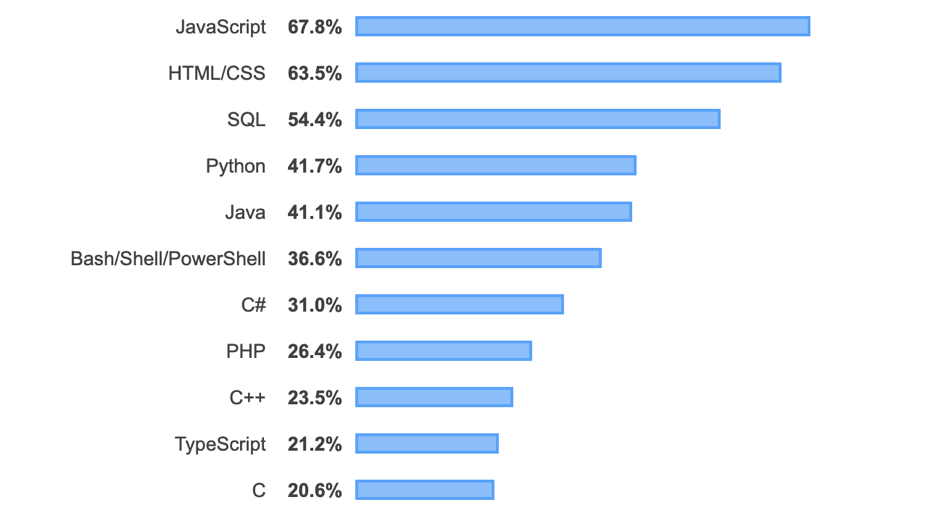
\includegraphics{stackOverflow.png}%
\caption{Rangliste der beliebtesten Programmiersprachen }
\label{img:stackoverflowBild}
\end{figure}

25\% der Entwickler, die noch nicht mit Python gearbeitet haben, möchten diese Sprache gerne lernen. Diese Lernbereitschaft wurde in den letzten drei Jahren von keiner anderen Programmiersprache überboten \cite{stackoverflow}. Das spricht sehr dafür, dass Python in den kommenden Jahren immer weiter an Bedeutung gewinnen wird. In dieser wissenschaftlichen Ausarbeitung wurde Python verwendet, um einige der Graphen und Kennlinien zu erzeugen. 

\section{Opjektorientierte Programmierung in Python}

Im folgendem wird die objektorientierte Programmierung in Python anhand der vier Grundprinzipien, Generalisierung, Vererbung, Kapselung und Polymorphismus erläutert. 

\subsection{Klasse}

\subsection{Generalisierung}

\subsection{Vererbung}
\subsection{Kapselung}
\subsection{Polymorphismus}
